\documentclass[11pt]{article}

% ---------------------------------------------------------------
% A benchmark generator of realistic logistic transport networks
% with nonlinear edge costs and transshipment capacities.
% ---------------------------------------------------------------

\usepackage[utf8]{inputenc}
\usepackage[T1]{fontenc}
\usepackage{lmodern}
\usepackage[margin=1in]{geometry}
\usepackage{amsmath,amssymb}
\usepackage{mathtools}
\usepackage{graphicx}
\usepackage{booktabs}
\usepackage{array}
\usepackage{caption}
\usepackage{subcaption}
\usepackage{enumitem}
\usepackage[hidelinks]{hyperref}
\usepackage{xcolor}

\captionsetup{font=small,labelfont=bf}
\setlength{\parskip}{2pt}

\newcommand{\Vv}{V}
\newcommand{\E}{E}
\newcommand{\Real}{\mathbb{R}}

\title{\textbf{A Benchmark Generator of Realistic Logistic Transport Networks
with Nonlinear Edge Costs and Transshipment Capacities}}

\author{Varvara Kovaleva \and Alexander Ponomarenko\\[2pt]
\small Laboratory of Algorithms and Technologies for Network Analysis,,\\
\small National Research University Higher School of Economics, Nizhny Novgorod, Russia}

\date{}

\begin{document}
\maketitle

\begin{abstract}
\noindent
Optimisation over logistic transport networks---routing many commodities at
minimum joint cost of vehicle movements and transshipment at intermediate
storages---lacks a public benchmark when edge costs are \emph{nonlinear}
(freight travels in fixed-capacity vehicles) and storages have \emph{hard
reload-capacity} limits. We close this gap with a generator of synthetic
logistic networks, calibrated on real road graphs of nine European countries,
five U.S.\ states and the European part of Russia extracted from
OpenStreetMap. The generator reproduces the structural signatures of
upper-level distribution networks---near-planar topology, low vertex degree,
short edges and large diameters---by combining four well-grounded ingredients:
Zipf-distributed city sizes, a spatial-network construction model that trades
edge-building cost against routing convenience, storage capacities driven by
population and betweenness centrality, and a doubly constrained gravity model
for demand. We release 34 fully synthetic instances ($10$--$150$ storages) and
15 real-geometry instances, in an open, self-describing file format. An
empirical characterisation, computed directly from the released files, shows
that the synthetic instances match the real ones across degree, diameter,
edge-length, rank--size and demand statistics, confirming that the corpus is a
faithful and reusable testbed for exact and heuristic solvers.
\end{abstract}

\noindent\textbf{Keywords:} benchmark generation; logistic networks; spatial
networks; multi-commodity flow; gravity model; Zipf's law; synthetic data.

\section{Introduction}

Planning commodity flows between distribution centres is a core problem for
logistic operators, and its realistic variants are computationally hard. Two
features make real instances especially difficult. First, the cost of using a
road is \emph{nonlinear} in the volume carried: goods move in vehicles of fixed
capacity, so the billed quantity is the integer number of vehicles obtained by
rounding the carried volume up to a vehicle capacity. Second, every storage has
a finite \emph{transshipment capacity}, an upper bound on the volume that can be
unloaded, stored and reloaded there. The resulting model is a capacitated
multi-commodity flow problem with a step-wise vehicle cost---NP-hard, and
sensitive to the topology and the demand pattern of the underlying network.

Progress on solvers for such problems is hampered by the absence of suitable
public benchmarks. Classical multi-commodity flow libraries do not carry
node-level transshipment capacities, per-unit reload costs or vehicle-induced
nonlinear edge costs, and they rarely reflect the geographic structure of
country-scale distribution networks. Moreover, the true locations of commercial
distribution centres are proprietary. Researchers are therefore left to test on
either toy graphs or ad-hoc random graphs whose structure differs sharply from
real transport networks, which undermines the external validity of any
comparison.

\paragraph{Contributions.}
This paper introduces a generator and an accompanying instance corpus designed
to remove that obstacle. Specifically, we
\begin{enumerate}[leftmargin=1.4em,itemsep=1pt,topsep=2pt]
\item define precisely the data an instance of the problem must contain
      (Section~\ref{sec:problem});
\item analyse real road graphs extracted from OpenStreetMap and distil the
      structural properties a realistic generator must reproduce
      (Section~\ref{sec:real});
\item present a five-stage generation pipeline combining Zipf city sizes, a
      spatial-network budget model, centrality-driven storage capacities, and a
      gravity demand model (Section~\ref{sec:pipeline});
\item describe the released benchmark and its open file format
      (Section~\ref{sec:benchmark}); and
\item characterise the corpus empirically, directly from the released files,
      showing that synthetic and real-geometry instances are statistically
      consistent (Section~\ref{sec:char}).
\end{enumerate}
The optimisation algorithm we developed for this problem is reported separately;
here the focus is the data and its fidelity.

\section{The optimisation problem an instance must support}
\label{sec:problem}

To fix the data requirements, we briefly state the target problem. The network
is a directed graph $G=(\Vv,\E)$ of storages $\Vv$ and roads $\E$. A set of
transportation requests (commodities) $K$ is given; each $k\in K$ has an origin
$s_k$, a destination $t_k$ and a demand $d_k\in\Real_+$. Each storage $v$ has a
per-unit reload cost $f_v\in\Real_+$ and a maximum transshipment volume
$W_v\in\Real_+$; each edge $e$ has a per-vehicle traversal cost $c_e\in\Real_+$;
and vehicles have a fixed capacity $C$. Writing $x^k_e$ for the flow of
commodity $k$ on edge $e$ and $y_e\in\mathbb{Z}_+$ for the number of vehicles on
$e$, the problem minimises movement plus reload cost,
\begin{equation}
\min\ \sum_{e\in \E} c_e\,y_e
 \;+\!\!\sum_{k\in K}\sum_{\substack{v\neq s_k,\,v\neq t_k}}\;
 \sum_{e\in\delta^-(v)} f_v\,x^k_e,
\end{equation}
subject to flow conservation, the vehicle-capacity coupling
$\sum_{k} x^k_e\le C\,y_e$ for all $e$, and the storage-capacity bound
$\sum_{k}\sum_{e\in\delta^-(v)} x^k_e\le W_v$ for all transit $v$.

Consequently, a complete instance must specify: a weighted graph with vertex
coordinates; per-storage reload cost $f_v$ and capacity $W_v$; per-edge cost
$c_e$ (here proportional to road length); a vehicle capacity $C$; and an
origin--destination demand set $\{(s_k,t_k,d_k)\}$. The generator below produces
exactly these objects, together with the auxiliary data (populations, shortest
distances) used to derive them.

\section{Structural properties of real networks}
\label{sec:real}

Since the locations of real distribution centres are not public, we calibrate on
city locations, populations and highways from OpenStreetMap~\cite{osm}, for nine
European countries of varying size, five large U.S.\ states, and the European
part of Russia. From the raw highway graph and city list we aggregate nearby
road endpoints into nodes, select cities greedily by descending population
subject to a minimum spacing, attach each retained city to a nearby high-degree
road node (junctions are economical places for a centre), and finally simplify
the graph so that each retained centre is joined to others by edges equal to the
shortest stop-free paths. Edges are then treated as straight segments of
Euclidean length, as modelling the true road geometry would over-complicate
synthesis without materially changing the network structure.

Three structural signatures emerge robustly and become the design targets of the
generator. (i)~The edge-length distribution is dominated by short edges, with
very few long edges between distant nodes. (ii)~Hop diameters are large relative
to size (Table~\ref{tab:diam}); together with the edge-length distribution this
indicates the \emph{opposite} of a small-world structure---routes between distant
nodes pass through many short edges. (iii)~The mean vertex degree is low: about
$3.4$ across all calibration graphs, well below the planar upper bound of $6$, so
the networks are essentially planar (drawable without edge crossings). These
properties are characteristic of spatial transport networks~\cite{barthelemy2011}
and any plausible generator must reproduce them.

\begin{table}[t]
\centering
\caption{Hop diameter and size of representative calibration graphs.}
\label{tab:diam}
\small
\begin{tabular}{lcc@{\hskip 1.4em}lcc}
\toprule
Network & diam & $|V|$ & Network & diam & $|V|$\\
\midrule
Belgium & 5 & 16 & Italy & 11 & 46\\
Denmark & 5 & 11 & Sweden & 11 & 45\\
Germany & 8 & 49 & United Kingdom & 9 & 42\\
Spain & 9 & 59 & California & 12 & 39\\
Europe Russia & 16 & 90 & Texas & 10 & 58\\
\bottomrule
\end{tabular}
\end{table}

\section{The generation pipeline}
\label{sec:pipeline}

Given a desired number of storages $k$, the generator proceeds in five stages.

\subsection{City sizes via Zipf's law}
A pool of cities (several times larger than $k$) is created with sizes following
Zipf's law~\cite{gabaix1999},
\begin{equation}
size_i=\frac{P}{rank_i^{\alpha}}, \qquad rank_i=1,2,\dots,N,
\end{equation}
where $P$ is the largest city's size and small multiplicative noise is added for
realism. Across the calibration regions the fitted exponent clusters near
$\alpha\approx0.974$, so the generator draws $\alpha\sim\mathcal{N}(0.974,0.06)$,
the largest population from $(9,11)\cdot 10^4\,k$, and a city count of $k$ times
a random integer in $[8,12]$.

\subsection{Spatial layout}
The $k$ city clusters are placed on a square map with \texttt{make\_blobs}
(cluster standard deviation about $1/15$ of the map side), seeding the largest
city in each cluster; this imitates the real pattern of smaller towns
surrounding a large city. Nearby cities are then aggregated into storages exactly
as in the calibration step, and each storage inherits the summed population of
its nearest cities. The minimum spacing between storages is a random value in
$[80,100]$ and the map side scales as that spacing times $k^{0.8}$.

\subsection{Topology via a spatial-network budget model}
Following Gastner and Newman~\cite{gastner2006}, edges are chosen to balance
construction cost against routing convenience. Construction cost is the total
edge length $\sum_{(i,j)} d_{ij}$ (Euclidean, in km), while the routing
``effective distance'' of an edge is
\begin{equation}
L_{ij}=\lambda\,d_{ij}+(1-\lambda)\cdot 1, \qquad 0\le\lambda\le1,
\end{equation}
so that $\lambda=1$ measures routes in kilometres and $\lambda=0$ in hop count.
Starting from a minimum spanning tree (which both guarantees connectivity and
sets the budget reference), edges are added within a budget---a coefficient times
the MST cost---so as to minimise mean pairwise effective distance, an
optimisation we solve by simulated annealing. Matching the diameter, mean edge
length and mean degree of the calibration graphs yields
$\lambda\sim\mathcal{N}(0.263,0.15)$ and budget coefficient
$\sim\mathcal{N}(2.56,0.6)$: a small budget admits only a few long edges among
many short ones, exactly the observed real pattern. Each edge is duplicated in
reverse with length differing by at most one percent, and per-vehicle cost is
$c_e=cost_{km}\cdot dist_e$ with $cost_{km}=5$.

\subsection{Storage capacities and reload costs}
A storage's transshipment capacity should reflect both the demand it serves
(population) and the through-flow it attracts. The latter correlates strongly
with betweenness centrality~\cite{barthelemy2011,kirkley2018}, so capacity is
\begin{equation}
maxoverload_i=l\cdot population_i^{\gamma}\,(1+\alpha\,\tilde b_i),
\end{equation}
where $\tilde b_i$ is normalised betweenness, with $l=1,\gamma=0.5,\alpha=1.2$ and
a floor $mincapacity=100$ (capacities are adapted so at least $10\%$ fall below
the floor). Reload costs decrease with capacity, reflecting economies of scale:
\begin{equation}
cost_i=\frac{\kappa}{maxoverload_i^{\delta}}, \qquad \kappa=500,\ \delta=1.
\end{equation}

\subsection{Demand via a doubly constrained gravity model}
The origin--destination matrix uses a doubly constrained gravity
model~\cite{wilson1967},
\begin{equation}
T_{ij}=A_i\,O_i\,B_j\,D_j\,f(dist_{ij}), \qquad f(dist)=dist^{-\beta},\ \beta=1,
\end{equation}
where the marginals $O_i,D_j$ are proportional to served population (plus small
noise), $dist_{ij}$ is the shortest network distance, and the balancing factors
$A_i,B_j$ enforce $\sum_j T_{ij}=O_i$ and $\sum_i T_{ij}=D_j$, computed by
iterative fitting. Total flow is scaled to a few times the total storage
capacity so that the capacity constraints bind. Finally $25\%$ of requests are
dropped with probability proportional to their volume, so that not every pair
exchanges goods, as in real demand matrices.

\section{The benchmark instances}
\label{sec:benchmark}

The corpus has two parts. The \textbf{synthetic} set, produced fully by the
pipeline, contains $34$ instances: $10$ with $10$ storages, $7$ each with $20$
and $30$, $5$ with $50$, $3$ with $100$ and $3$ with $150$. The
\textbf{real-geometry} set contains $15$ instances built on the calibration
regions ($11$ to $90$ storages): the vertex coordinates and populations come from
OpenStreetMap, while edge costs, storage capacities, reload costs and demand are
generated by stages~3--5 above. Together this spans $10$ to $150$ storages and
$67$ to over $16{,}000$ commodities.

Each instance is a directory of plain, self-describing files
(Table~\ref{tab:format}): an undirected weighted graph in GraphML with vertex
coordinates, a per-storage table of reload cost and capacity, a city
position/population table, the demand requests, a precomputed shortest-distance
matrix, and a parameter file recording the random seed and every generation
parameter, so each instance is exactly reproducible.

\begin{table}[t]
\centering
\caption{File format of a benchmark instance.}
\label{tab:format}
\small
\begin{tabular}{ll}
\toprule
File & Contents\\
\midrule
\texttt{graph.graphml}        & weighted graph; node \texttt{x,y}; edge \texttt{weight} (road length)\\
\texttt{offices.csv}          & \texttt{office\_id, transfer\_price} ($f_v$), \texttt{transfer\_max} ($W_v$)\\
\texttt{pos\_pop.csv}         & city/storage \texttt{x, y, population}\\
\texttt{reqs.csv}             & demand requests \texttt{src, dst, volume} ($s_k,t_k,d_k$)\\
\texttt{distance\_matrix.csv} & all-pairs shortest road distances\\
\texttt{data.txt}             & random seed and all generation parameters\\
\bottomrule
\end{tabular}
\end{table}

\section{Empirical characterisation}
\label{sec:char}

We now characterise the corpus using statistics computed directly from the
released files, to verify that the synthetic instances reproduce real network
structure. Tables~\ref{tab:syn} and~\ref{tab:real} summarise the per-size
synthetic aggregates and the individual real networks; all figures below pool
every instance unless stated otherwise.

\begin{table}[t]
\centering
\caption{Synthetic instances aggregated by size ($n$ instances per size):
mean degree, hop diameter, mean edge length, mean storage capacity $\bar W$,
mean reload cost $\bar f$, number of commodities $|K|$ and mean demand
$\bar d$.}
\label{tab:syn}
\small
\begin{tabular}{ccccccccc}
\toprule
$|V|$ & $n$ & $deg_{\text{mean}}$ & diam & $dist_{\text{mean}}$ & $\bar W$ & $\bar f$ & $|K|$ & $\bar d$\\
\midrule
10  & 10 & 3.68 & 3.3  & 189.5 & 266.0 & 2.63 & 67    & 153.4\\
20  & 7  & 4.06 & 5.3  & 261.6 & 230.4 & 2.75 & 285   & 56.7\\
30  & 7  & 3.25 & 7.9  & 261.9 & 199.1 & 3.00 & 652   & 36.1\\
50  & 5  & 3.18 & 9.4  & 304.8 & 182.8 & 3.22 & 1837  & 21.9\\
100 & 3  & 3.05 & 12.0 & 481.0 & 178.6 & 3.27 & 7425  & 17.2\\
150 & 3  & 3.15 & 18.7 & 477.0 & 177.4 & 3.30 & 16762 & 12.4\\
\bottomrule
\end{tabular}
\end{table}

\begin{table}[t]
\centering
\caption{Real-geometry instances: structural and instance statistics computed
from the released files. $W_{\text{sum}}$ is total storage capacity,
$d_{\text{sum}}$ total demand.}
\label{tab:real}
\small
\begin{tabular}{lcccccccc}
\toprule
Network & $|V|$ & $deg_{\text{mean}}$ & diam & $dist_{\text{mean}}$ & $W_{\text{sum}}$ & $\bar f$ & $|K|$ & $d_{\text{sum}}$\\
\midrule
Denmark        & 11 & 2.55 & 5  & 130.4 & 3294  & 2.35 & 82   & 8323\\
Belgium        & 16 & 3.12 & 5  & 76.3  & 5703  & 2.11 & 180  & 15717\\
Netherlands    & 18 & 3.67 & 5  & 97.3  & 4694  & 2.73 & 229  & 11605\\
Hungary        & 19 & 2.74 & 7  & 103.3 & 4566  & 3.26 & 256  & 20566\\
Ohio USA        & 22 & 3.73 & 6  & 106.8 & 7371  & 2.58 & 346  & 22994\\
Georgia USA     & 24 & 3.75 & 7  & 112.4 & 7720  & 2.57 & 414  & 34832\\
Illinois USA    & 28 & 3.50 & 6  & 109.5 & 10292 & 2.53 & 567  & 24337\\
California USA   & 39 & 2.56 & 12 & 138.5 & 36544 & 1.48 & 1111 & 114359\\
United Kingdom & 42 & 4.19 & 9  & 171.2 & 24109 & 1.75 & 1291 & 77119\\
Sweden         & 45 & 3.42 & 11 & 225.4 & 21373 & 1.83 & 1485 & 85688\\
Italy          & 46 & 3.61 & 11 & 134.7 & 14288 & 2.40 & 1552 & 61953\\
Germany        & 49 & 5.39 & 8  & 206.8 & 14276 & 2.54 & 1764 & 43705\\
Texas USA       & 58 & 3.00 & 10 & 138.5 & 27767 & 2.31 & 2479 & 110540\\
Spain          & 59 & 4.14 & 9  & 151.5 & 19789 & 2.38 & 2566 & 77666\\
Europe Russia  & 90 & 4.27 & 16 & 394.2 & 42492 & 2.03 & 6007 & 132570\\
\bottomrule
\end{tabular}
\end{table}

\paragraph{Topology.}
Figure~\ref{fig:layouts} shows a synthetic instance beside the Spain network:
both display the same near-planar, locally clustered structure with mostly short
edges. The degree distribution (Figure~\ref{fig:degree}) is tightly concentrated
below the planar bound of $6$, with synthetic and real means of $3.4$ and $3.5$
respectively. The edge-length distribution (Figure~\ref{fig:edgelen}), normalised
by each graph's largest pairwise distance, is right-skewed and dominated by short
edges in both populations. Hop diameter grows with size faster than the
$\sqrt{|V|}$ reference (Figure~\ref{fig:diameter}), confirming the non-small-world
character; synthetic and real points overlap throughout.

\begin{figure}[t]
\centering
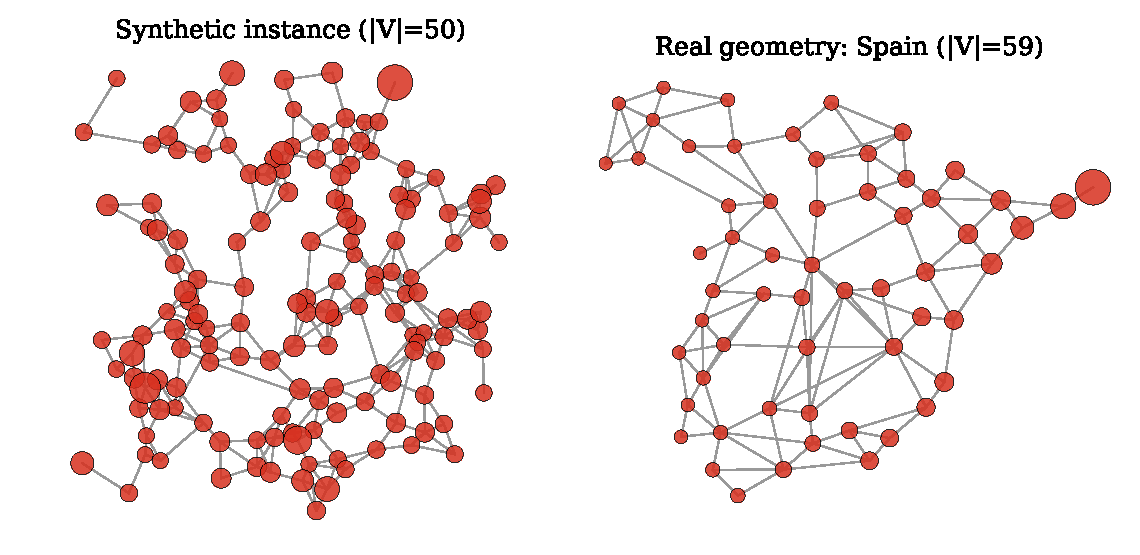
\includegraphics[width=0.96\textwidth]{dfigs/layouts.pdf}
\caption{Generated layouts. Left: a fully synthetic instance ($|V|=50$). Right: a
real-geometry instance (Spain, $|V|=59$). Node area encodes storage capacity.
Both share the near-planar, short-edge structure of real transport networks.}
\label{fig:layouts}
\end{figure}

\begin{figure}[t]
\centering
\begin{subfigure}{0.49\textwidth}
  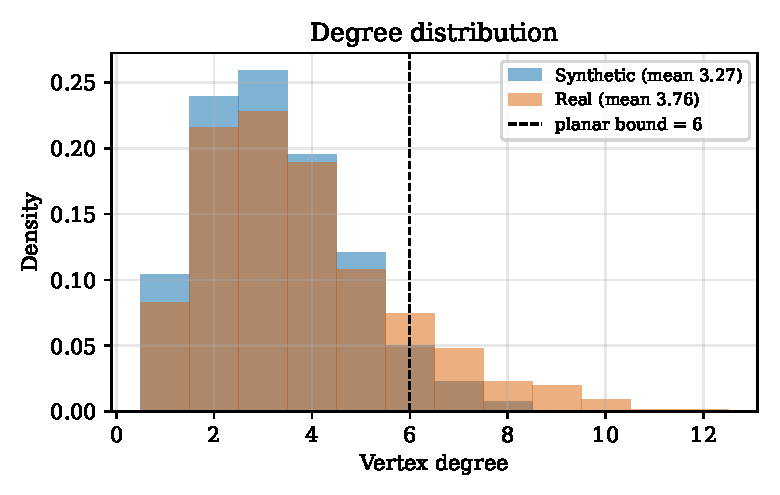
\includegraphics[width=\linewidth]{dfigs/degree.pdf}
  \caption{Degree distribution.}
  \label{fig:degree}
\end{subfigure}\hfill
\begin{subfigure}{0.49\textwidth}
  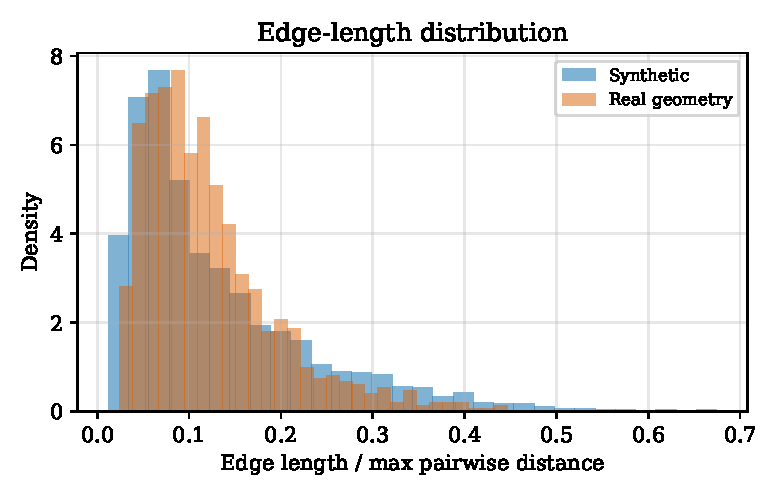
\includegraphics[width=\linewidth]{dfigs/edgelen.pdf}
  \caption{Edge-length distribution.}
  \label{fig:edgelen}
\end{subfigure}
\caption{Pooled topological distributions over all instances. Synthetic and
real-geometry instances are closely aligned, and both stay below the planar
degree bound and are dominated by short edges.}
\label{fig:topodist}
\end{figure}

\begin{figure}[t]
\centering
\begin{subfigure}{0.49\textwidth}
  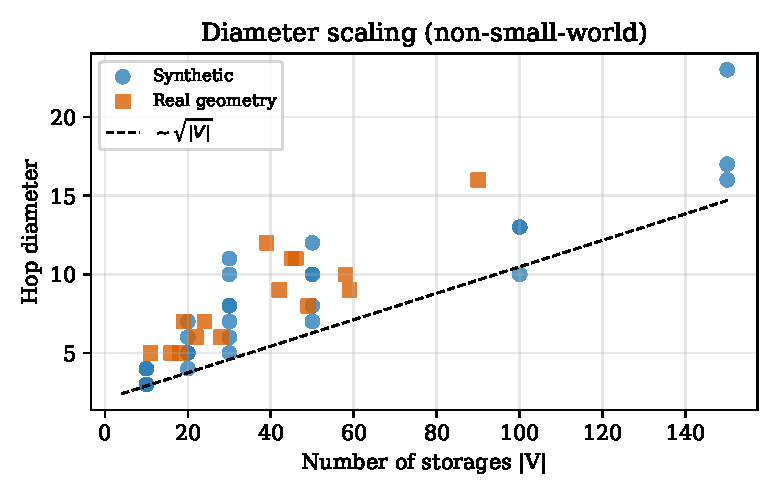
\includegraphics[width=\linewidth]{dfigs/diameter.pdf}
  \caption{Diameter vs.\ size.}
  \label{fig:diameter}
\end{subfigure}\hfill
\begin{subfigure}{0.49\textwidth}
  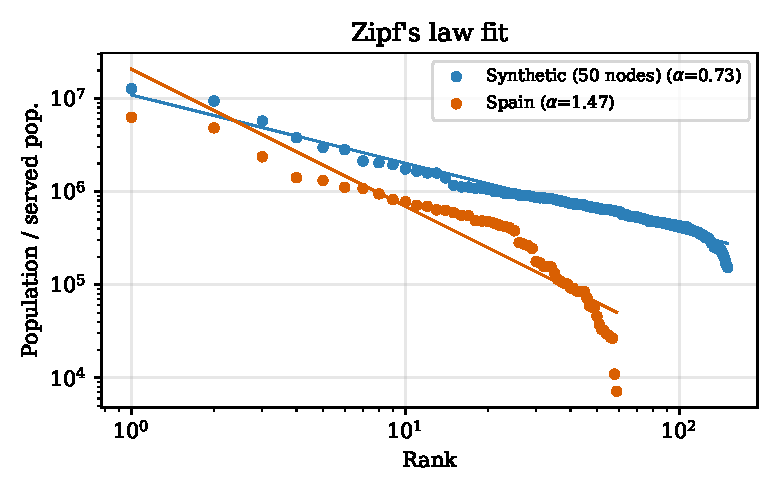
\includegraphics[width=\linewidth]{dfigs/zipf.pdf}
  \caption{Rank--size (Zipf) relation.}
  \label{fig:zipf}
\end{subfigure}
\caption{Left: hop diameter grows faster than $\sqrt{|V|}$ for both populations,
i.e.\ networks are not small-world. Right: the rank--size relation of storage
populations is approximately log-linear, as Zipf's law prescribes.}
\label{fig:diamzipf}
\end{figure}

\paragraph{Populations and instance parameters.}
The rank--size relation of storage populations (Figure~\ref{fig:zipf}) is
approximately log-linear on log--log axes for both a synthetic instance and
Spain, consistent with the Zipf prior used in stage~1. Storage capacities and
reload costs follow the intended inverse relationship---larger storages reload
more cheaply (Figure~\ref{fig:capdemand}, left)---and request volumes are
right-skewed with many small and few large shipments
(Figure~\ref{fig:capdemand}, right), as produced by the gravity model.

\begin{figure}[t]
\centering
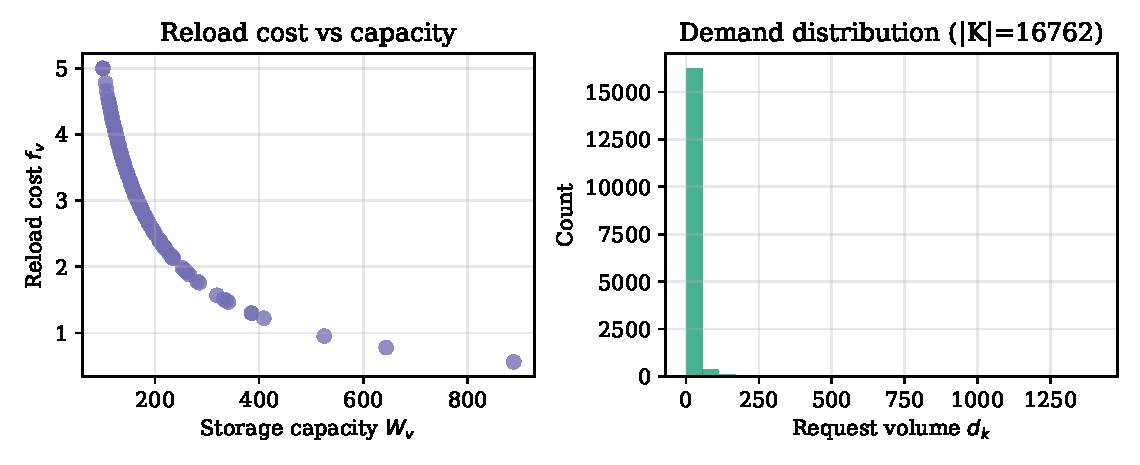
\includegraphics[width=0.96\textwidth]{dfigs/capdemand.pdf}
\caption{Instance parameters for a synthetic $|V|=50$ network. Left: reload cost
$f_v$ decreases with storage capacity $W_v$ (economies of scale). Right:
right-skewed distribution of request volumes $d_k$ from the gravity model.}
\label{fig:capdemand}
\end{figure}

\paragraph{Consistency.}
Across every statistic examined---degree, diameter scaling, edge-length shape,
rank--size slope, and the capacity/demand distributions---the synthetic and
real-geometry instances behave alike (cf.\ Tables~\ref{tab:syn}--\ref{tab:real}
and Figures~\ref{fig:topodist}--\ref{fig:capdemand}). This is the central
validation result: the generator does not merely produce hard instances, it
produces instances whose structure is statistically indistinguishable, in the
measured respects, from networks built on real geography. Solvers tuned on the
synthetic set can therefore be expected to transfer to real-world inputs.

\section{Reproducibility and tooling}
\label{sec:repro}

Every instance records its random seed and full parameter set in
\texttt{data.txt}, so the corpus regenerates exactly. To inspect instances and
solver outputs we provide an interactive web application (Streamlit/Plotly) that
loads any instance from the corpus and draws the network on its geographic
layout, with node size encoding population and capacity, edge width encoding
vehicle load, and per-node congestion highlighted. The tool supports
per-commodity path inspection and aggregate statistics, and was used to produce
the layout views in this paper. The generator, the corpus and the viewer are
distributed together so that results on this benchmark are fully reproducible.

\section{Conclusion}

We have presented a generator and an open instance corpus for logistic network
flow problems with nonlinear, vehicle-induced edge costs and hard storage
transshipment capacities---a problem class for which no realistic public
benchmark previously existed. By calibrating on real road graphs and combining
Zipf city sizes, a spatial-network budget model, centrality-driven capacities and
a gravity demand model, the generator reproduces the near-planar topology, low
degree, short edges and large diameters of real upper-level distribution
networks. An empirical characterisation computed directly from the released files
shows that the $34$ synthetic and $15$ real-geometry instances are statistically
consistent across all measured properties, making the corpus a faithful and
reusable testbed. Natural extensions include time-dependent demand, multi-modal
edges, and stochastic capacities, each of which the parameterised pipeline can
accommodate.

\begin{thebibliography}{99}
\small
\bibitem{osm} OpenStreetMap. \url{https://www.openstreetmap.org} (accessed
2026-04-11).
\bibitem{gabaix1999} X.~Gabaix. Zipf's Law for Cities: An Explanation.
\textit{Quarterly Journal of Economics}, 114(3):739--767, 1999.
\bibitem{gastner2006} M.~T.~Gastner, M.~E.~J.~Newman. The spatial structure of
networks. \textit{The European Physical Journal B}, 49(2):247--252, 2006.
\bibitem{barthelemy2011} M.~Barth\'elemy. Spatial networks. \textit{Physics
Reports}, 499(1--3):1--101, 2011.
\bibitem{kirkley2018} A.~Kirkley, H.~Barbosa, M.~Barthelemy, G.~Ghoshal. From
networks to optimal higher-order models of complex systems. \textit{Nature
Physics}, 14:250--258, 2018.
\bibitem{wilson1967} A.~G.~Wilson. A statistical theory of spatial distribution
models. \textit{Transportation Research}, 1(3):253--269, 1967.
\bibitem{crainic2015} T.~G.~Crainic, M.~Gendreau, J.~M.~Farvolden.
Metaheuristics for Multi-Commodity Flow Problems. \textit{Parallel Computing},
41:1--15, 2015.
\bibitem{barnhart1998} C.~Barnhart, E.~L.~Johnson, G.~L.~Nemhauser,
M.~W.~P.~Savelsbergh, P.~H.~Vance. Branch-and-Price: Column Generation for
Solving Huge Integer Programs. \textit{Operations Research}, 46(3):316--329,
1998.
\end{thebibliography}

\end{document}
